% Provenance (never printed): see sources/outline_sources.md (Year 1: the general
% circulation of the atmosphere, Hadley, Ferrel and polar cells, the ITCZ, Walker cells,
% jet streams, the geostrophic wind, depressions and anticyclones). Exercise and problem
% values in the Book 3 scratch calculator calc/ch28.py; figures from
% figdata/bachelor-1/angular_momentum_wind.py, weather_map.py (an invented map) and
% general_circulation.py (NCEP-NCAR Reanalysis 1, long-term means 1991-2020, datasets
% bachelor-1-ncep-{uwnd-p,vwnd-p,uwnd-sfc,slp,prate-monthly}).
% Physics owns the Coriolis force and the hydrostatic relation (recalled). Book 1 (g8) gave
% the global winds, the convection cell, depressions and anticyclones, isobars and the
% rotation of the wind around them, in words: re-founded here with forces and data.
% ENSO and the monsoons are the Year 2 volume's; the thermal wind the Year 3 volume's.
\chapter{De algemene circulatie van de atmosfeer}\label{ch:b1:atmospheric-circulation}

De zeilschepen die van Europa en Afrika naar Amerika overstaken, vertrouwden op de passaatwinden, gestage oostenwinden van de tropen. Dichter bij de evenaar, binnen ongeveer vijf graden daarvan, vielen dezelfde winden stil, in de gordel van windstiltes en aanhoudende buien die zeelieden de doldrums noemden. Ver boven beide, ongeveer negen kilometer hoog, kunnen smalle rivieren van lucht, straalstromen genoemd, waaien met meer dan \qty{440}{km/h}. Dit hoofdstuk legt de drie uit: waarom lucht die over een roterende planeet beweegt waait uiteindelijk langs de isobaren in plaats van er dwars overheen, hoe het overschot van de tropen aan weerszijden van de evenaar een grote omkeercel aandrijft, en waarom de lucht die hoog boven de evenaar wegvloeit tot een westenwindstraal wordt.
% ledger: nos:trade-winds, nos:doldrums, noaajs:jet

\begin{omfigure}
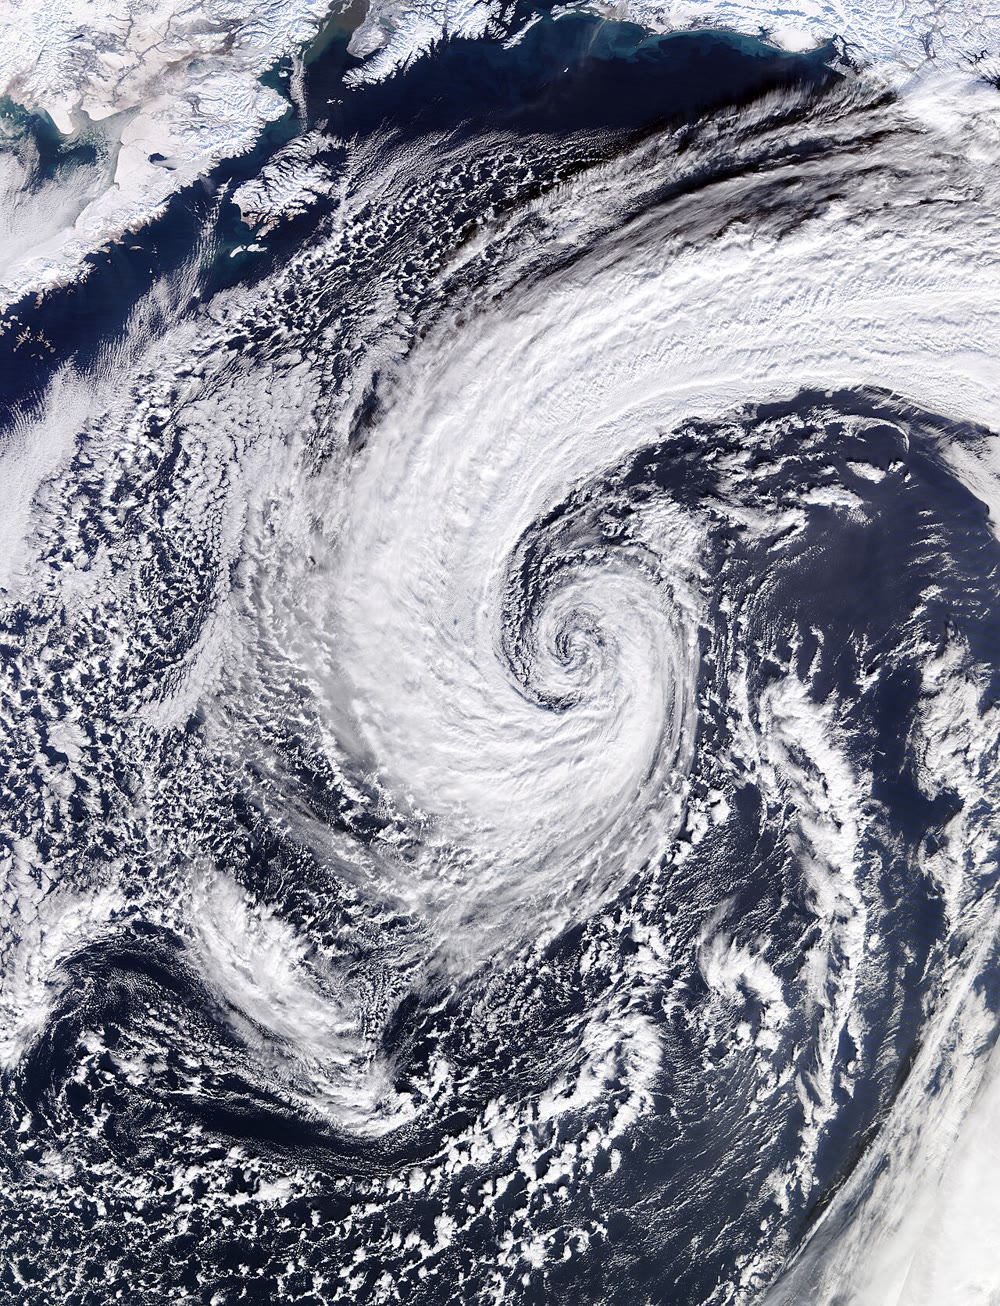
\includegraphics[width=0.5\linewidth]{images/book3/b1-alaska-low.jpg}

{\small Een extratropische \omterm{def:b1:atmospheric-circulation:cyclone}{cycloon} boven de Golf van Alaska op 28 januari 2018, gezien door het MODIS-instrument vanuit een baan; de met sneeuw bedekte kust van Alaska ligt linksboven, en het noorden is ongeveer omhoog. De wolkenbanden draaien tegen de klok in naar het centrum, zoals de lucht van een depressie op het noordelijk halfrond doet. (NASA, MODIS/LANCE, publiek domein, via Wikimedia Commons.)}
\label{fig:b1:atmospheric-circulation:alaska}
\end{omfigure}
% ledger: commons:alaska-low, nws:cyclone

\begin{recall}
De natuurkundeboeken geven de hydrostatische betrekking en de Coriolis-kracht: in een stelsel dat met hoeksnelheid $\vec\Omega$ roteert, voelt een lichaam van massa $m$ dat met snelheid $\vec v$ ten opzichte van het stelsel beweegt de schijnkracht $-2m\,\vec\Omega\times\vec v$, loodrecht op zijn beweging. Voor de aarde geldt $\Omega = 2\pi/T_\star$ met de sterrendag $T_\star = \qty{23.9345}{h}$, dat wil zeggen
$\Omega = \qty{7.292e-5}{rad.s^{-1}}$. Boek~1 beschreef de mondiale winden (de passaatwinden, de \omterm{def:b1:atmospheric-circulation:winds}{westenwinden}, de poolse oostenwinden), de convectiecel, depressies en anticyclonen, de isobaren van een weerkaart, en het draaien van de wind rond de centra. \Cref{ch:b1:fluid-envelopes-structure} gaf de \omterm{def:b1:fluid-envelopes-structure:standard-atmosphere}{standaardatmosfeer} en de \omterm{def:b1:fluid-envelopes-structure:lapse-rate}{droogadiabatische gradiënt}, en \cref{ch:b1:radiation-heat-transport} het poolwaartse warmtetransport dat de circulatie draagt.
% ledger: earth:Trot, nws:coriolis
\end{recall}

\section{Krachten op bewegende lucht}\label{sec:b1:atmospheric-circulation:forces}

Een \omterm{def:b1:fluid-envelopes-structure:parcel}{luchtpakketje} wordt geduwd door de druk van de lucht eromheen, getrokken door de zwaartekracht, afgeremd door wrijving nabij de grond en, gezien vanuit de roterende aarde, afgebogen door de Coriolis-kracht. Zwaartekracht en de verticale drukkracht houden elkaar bijna precies in evenwicht: dit is de hydrostatische betrekking. Het weer wordt gemaakt door de krachten die in het horizontale vlak overblijven.

\begin{definition}[Drukgradiëntkracht]\label{def:b1:atmospheric-circulation:pgf}
De \emph{drukgradiëntkracht}\index{drukgradiëntkracht} is de netto kracht die door de druk van het omringende fluïdum op een pakketje fluïdum wordt uitgeoefend. Per eenheid van massa is zij $-(1/\rho)\nabla p$, waarin $\rho$ de dichtheid is en $\nabla p$ de drukgradiënt: zij wijst van hoge naar lage druk, dwars op de isobaren.
\end{definition}
% ledger: nws:geostrophic

\begin{proposition}[De drukgradiëntkracht]\label{prop:b1:atmospheric-circulation:pgf}
Op een pakketje van volume $\mathrm dV$ en dichtheid $\rho$ oefent de druk van het omringende fluïdum de kracht $-\nabla p\,\mathrm dV$ uit, een versnelling $-(1/\rho)\nabla p$.
\end{proposition}

\begin{proof}
Neem een klein doosje met ribben $\mathrm dx$, $\mathrm dy$, $\mathrm dz$ langs de assen. Op het vlak bij $x$ duwt de druk in de $+x$-richting met de kracht $p(x)\,\mathrm dy\,\mathrm dz$; op het vlak bij $x + \mathrm dx$, in de $-x$-richting met $p(x + \mathrm dx)\,\mathrm dy\,\mathrm dz$. De netto kracht langs $x$ is $[p(x) - p(x + \mathrm dx)]\,\mathrm dy\,\mathrm dz = -(\partial p/\partial
x)\,\mathrm dV$, en evenzo langs $y$ en $z$. Het totaal is $-\nabla p\,
\mathrm dV$; delen door de massa $\rho\,\mathrm dV$ geeft de versnelling.
\end{proof}

Een uniforme druk oefent geen netto kracht uit: alleen de verschillen duwen. Op een weerkaart wordt de horizontale gradiënt afgelezen aan de isobaren: haar grootte is de drukstap tussen twee isobaren gedeeld door hun afstand. Voor isobaren \qty{4}{hPa} uit elkaar en \qty{400}{km} uit elkaar aan zeeniveau, waar $\rho \approx \qty{1.225}{kg.m^{-3}}$, is de versnelling $400/(1.225 \times \num{4e5}) = \qty{8.2e-4}{m.s^{-2}}$, minder dan een tienduizendste van $g$, maar genoeg om lucht van stilstand tot \qty{10}{m/s} te brengen in drie en een half uur.
% ledger: ussa76:sea-level

De lucht voelt de Coriolis-kracht omdat zij wordt waargenomen vanaf de draaiende aarde. Haar horizontale deel hangt van de \omterm{def:b1:spherical-astronomy:geographic}{breedtegraad} af via één getal.

\begin{definition}[Coriolisparameter]\label{def:b1:atmospheric-circulation:coriolis-parameter}
De \emph{Coriolisparameter}\index{Coriolisparameter} op \omterm{def:b1:spherical-astronomy:geographic}{breedtegraad} $\varphi$ is $f = 2\Omega\sin\varphi$, waarin $\Omega$ de hoeksnelheid van de aarde is. Zij is positief op het noordelijk halfrond, negatief op het zuidelijke, nul aan de evenaar, en het grootst aan de polen, $2\Omega = \qty{1.458e-4}{s^{-1}}$.
\end{definition}
% ledger: earth:Trot

\begin{proposition}[Horizontale Coriolis-versnelling]\label{prop:b1:atmospheric-circulation:coriolis}
Voor een horizontale wind $\vec v$ op \omterm{def:b1:spherical-astronomy:geographic}{breedtegraad} $\varphi$ is het horizontale deel van de Coriolis-versnelling $-f\,\vec k\times\vec v$, waarin $\vec k$ de opwaartse verticale is: zij heeft de grootte $|f|\,|\vec v|$ en wijst loodrecht op de wind, naar rechts op het noordelijk halfrond en naar links op het zuidelijke.
\end{proposition}

\begin{proof}
Gebruik lokale assen $x$ oost, $y$ noord, $z$ omhoog. De rotatievector van de aarde ligt in het meridiaanvlak, op de hoek $\varphi$ boven de noordelijke horizon: $\vec\Omega =
\Omega(0, \cos\varphi, \sin\varphi)$. Voor $\vec v = (u, v, 0)$,
\[
  \vec\Omega\times\vec v = \Omega\,(-v\sin\varphi,\ u\sin\varphi,\ -u\cos\varphi),
  \qquad -2\vec\Omega\times\vec v = (f v,\ -f u,\ 2\Omega u\cos\varphi).
\]
Aangezien $\vec k\times\vec v = (-v, u, 0)$, is het horizontale deel $(fv, -fu)$ gelijk aan
$-f\,\vec k\times\vec v$. De vector $\vec k\times\vec v$ is $\vec v$ gedraaid over
\ang{90} tegen de klok in gezien van boven; haar tegengestelde is $\vec v$ rechtsom gedraaid, naar rechts, wanneer $f > 0$, en naar links wanneer $f < 0$.
\end{proof}
% ledger: earth:Trot

De verticale component, $2\Omega u\cos\varphi$, is hoogstens \qty{1.5e-3}{m.s^{-2}} voor een wind van \qty{10}{m/s}, ongeveer \num{1.5e-4} van $g$: de hydrostatische balans neemt haar op. De horizontale component, hoe klein ook, heeft geen tegenhanger in de vrije atmosfeer boven de wrijvingslaag, en binnen enkele uren bepaalt zij de wind.

Nabij de grond wrijft de lucht ook tegen het oppervlak. In de onderste kilometer, de wrijvingslaag van de meteorologen, verandert wrijving zowel de snelheid als de richting van de wind; turbulente wervels voeren de weerstand van het oppervlak omhoog, en de kracht werkt ruwweg tegen de wind in en groeit ermee. Erboven, in de vrije atmosfeer, is wrijving klein.
% ledger: nws:friction-layer

\section{De geostrofische wind}\label{sec:b1:atmospheric-circulation:geostrophic}

\begin{definition}[Geostrofisch evenwicht, geostrofische wind]\label{def:b1:atmospheric-circulation:geostrophic}
Een horizontale stroming is in \emph{geostrofisch evenwicht}\index{geostrofisch evenwicht} wanneer haar \omterm{def:b1:atmospheric-circulation:pgf}{drukgradiëntkracht} en haar Coriolis-kracht elkaar opheffen. De \emph{geostrofische
wind}\index{geostrofische wind} $\vec v_g$ is de wind die dit evenwicht voor een gegeven drukveld bereikt: $-(1/\rho)\nabla p - f\,\vec k\times\vec v_g = \vec 0$.
\end{definition}
% ledger: nws:geostrophic

\begin{theorem}[De geostrofische wind]\label{thm:b1:atmospheric-circulation:geostrophic}
Buiten de evenaar geldt
\[
  \vec v_g = \frac{1}{\rho f}\,\vec k\times\nabla p, \qquad
  |\vec v_g| = \frac{|\nabla p|}{\rho\,|f|} .
\]
De \omterm{def:b1:atmospheric-circulation:geostrophic}{geostrofische wind} waait langs de isobaren, sneller waar zij dichter bij elkaar liggen. Op het noordelijk halfrond houdt zij de lage druk aan haar linkerhand; op het zuidelijke
halfrond, aan haar rechterhand.
\end{theorem}

\begin{proof}
Voor een horizontale vector $\vec w$ geldt $\vec k\times(\vec k\times\vec w) = -\vec w$. Door $\vec k\times$ toe te passen op het evenwicht $f\,\vec k\times\vec v_g = -(1/\rho)\nabla p$ volgt $-f\vec v_g = -(1/\rho)\,\vec k\times\nabla p$, dus de formule, geldig waar
$f \neq 0$. Aangezien $\vec k\times\nabla p$ loodrecht op $\nabla p$ staat, staat de wind loodrecht op de gradiënt, dat wil zeggen langs de isobaren; haar grootte is $|\nabla
p|/(\rho|f|)$. De vector $\vec k\times\nabla p$ is de gradiënt over \ang{90} tegen de klok in gedraaid. Als men in haar richting kijkt, ligt de gradiënt, die naar hoge druk wijst, rechts, dus ligt lage druk links; voor $f > 0$ heeft de wind de richting van $\vec k\times\nabla p$, voor $f < 0$ de tegengestelde.
\end{proof}

\begin{example}[Een wind afgelezen aan de isobaren]\label{ex:b1:atmospheric-circulation:geostrophic}
Op \ang{50} N is $f = 2 \times \num{7.292e-5} \times \sin\ang{50} = \qty{1.117e-4}{s^{-1}}$.
Isobaren \qty{4}{hPa} uit elkaar en \qty{400}{km} uit elkaar geven $|\nabla p| = 400/\num{4e5} =
\qty{1.0e-3}{Pa.m^{-1}}$ en, met $\rho = \qty{1.225}{kg.m^{-3}}$, een \omterm{def:b1:atmospheric-circulation:geostrophic}{geostrofische
wind} van $\num{1.0e-3}/(1.225 \times \num{1.117e-4}) = \qty{7.3}{m/s}$. Dezelfde
afstand op \ang{20} N, waar $f$ minder dan de helft zo groot is, zou
\qty{16.4}{m/s} geven.
\end{example}
% ledger: earth:Trot, ussa76:sea-level

De balans is niet onmiddellijk. Lucht die door een drukgradiënt in beweging wordt gezet, draait onder de Coriolis-kracht met de snelheid $f$, ongeveer eens in de $2\pi/f$, enkele zestien uur op \ang{50}; patronen die langer dan enkele uren aanhouden en groter zijn dan enkele honderden kilometers, zijn nagenoeg geostrofisch. Nabij de evenaar gaat $f$ naar nul, valt de formule uiteen, en zijn de winden van de diepe tropen niet geostrofisch.

\begin{omfigure}
\begin{tikzpicture}[>={Stealth[length=2.2mm]}, font=\scriptsize]
  % left panel: geostrophic balance
  \begin{scope}
    \draw[isobar] (-2.4,1.2) -- (2.4,1.2) node[right] {\qty{996}{hPa}};
    \draw[isobar] (-2.4,0) -- (2.4,0) node[right] {\qty{1000}{hPa}};
    \draw[isobar] (-2.4,-1.2) -- (2.4,-1.2) node[right] {\qty{1004}{hPa}};
    \node[pressure low] at (0,2.0) {L};
    \node[pressure high] at (0,-2.0) {H};
    \fill (0,0) circle (1.6pt);
    \draw[->, very thick, omThm] (0,0) -- (0,1.0);
    \node[omThm, anchor=east] at (-0.08,0.6) {drukgradiënt};
    \draw[->, very thick, omDef] (0,0) -- (0,-1.0);
    \node[omDef, anchor=east] at (-0.08,-0.6) {Coriolis};
    \draw[->, line width=1.6pt, black] (0,0) -- (1.9,0) node[above, pos=0.75] {wind $\vec v_g$};
    \node[anchor=north] at (0,-2.4) {zonder wrijving: geostrofisch};
  \end{scope}
  % right panel: with friction (alpha = 25 deg, V = Vg cos alpha)
  \begin{scope}[xshift=7.4cm]
    \draw[isobar] (-2.4,1.2) -- (2.4,1.2) node[right] {\qty{996}{hPa}};
    \draw[isobar] (-2.4,0) -- (2.4,0) node[right] {\qty{1000}{hPa}};
    \draw[isobar] (-2.4,-1.2) -- (2.4,-1.2) node[right] {\qty{1004}{hPa}};
    \node[pressure low] at (0,2.0) {L};
    \node[pressure high] at (0,-2.0) {H};
    \fill (0,0) circle (1.6pt);
    \draw[->, very thick, omThm] (0,0) -- (0,1.0);
    \node[omThm, anchor=east] at (-0.08,0.6) {drukgradiënt};
    \draw[->, very thick, omDef] (0,0) -- ({1.0*cos(25)*sin(25)},{-1.0*cos(25)*cos(25)});
    \node[omDef, anchor=west] at (0.42,-0.62) {Coriolis};
    \draw[->, very thick, omMeth] (0,0) -- ({-1.0*sin(25)*cos(25)},{-1.0*sin(25)*sin(25)})
      node[below left, inner sep=1pt] {wrijving};
    \draw[->, line width=1.6pt, black] (0,0) -- ({1.9*cos(25)*cos(25)},{1.9*cos(25)*sin(25)})
      node[above, inner sep=2pt] {wind $\vec v$};
    \draw[black!50, dashed] (0,0) -- (1.9,0);
    \draw[black!60] (1.0,0) arc[start angle=0, end angle=25, radius=1.0];
    \node[black!70] at (1.22,0.22) {$\alpha$};
    \node[anchor=north] at (0,-2.4) {met wrijving: trager, dwars op de isobaren};
  \end{scope}
\end{tikzpicture}

{\small Krachten op een \omterm{def:b1:fluid-envelopes-structure:parcel}{luchtpakketje} op het noordelijk halfrond, met lage druk naar het noorden. Links: in de vrije atmosfeer heffen de \omterm{def:b1:atmospheric-circulation:pgf}{drukgradiëntkracht} (rood) en de Coriolis-kracht (blauw) elkaar op, en waait de wind langs de isobaren met de lage druk aan haar linkerhand. Rechts: nabij de grond werkt wrijving (groen) tegen de wind in; de drie krachten houden elkaar alleen in evenwicht als de wind trager is en over een hoek $\alpha$ naar de lage druk wordt gedraaid (getekend voor $\alpha = \ang{25}$ en de weerstand van \cref{prop:b1:atmospheric-circulation:friction}).}
\label{fig:b1:atmospheric-circulation:balance}
\end{omfigure}

\begin{proposition}[Wrijving draait de wind naar lage druk]\label{prop:b1:atmospheric-circulation:friction}
Neem aan dat een stationaire horizontale wind $\vec v$ onderhevig is aan de \omterm{def:b1:atmospheric-circulation:pgf}{drukgradiëntkracht}, de Coriolis-kracht en een wrijvingskracht $-\vec v/\tau$, met $\tau > 0$, op een \omterm{def:b1:spherical-astronomy:geographic}{breedtegraad} waar $f > 0$. Dan steekt de wind de isobaren over naar lage druk onder de hoek $\alpha$ met $\tan\alpha = 1/(f\tau)$, en haar snelheid is $|\vec v| =
|\vec v_g|\cos\alpha$, minder dan de \omterm{def:b1:atmospheric-circulation:geostrophic}{geostrofische wind}.
\end{proposition}

\begin{proof}
Laat $V = |\vec v|$, $\hat v$ de eenheidsvector langs de wind en $\hat n$ de eenheidsvector loodrecht erop, naar haar linkerhand. Het evenwicht is $-(1/\rho)\nabla p - f\,
\vec k\times\vec v - \vec v/\tau = \vec 0$, en $\vec k\times\vec v = V\hat n$.
Langs $\hat v$: $-(1/\rho)\,\nabla p\cdot\hat v = V/\tau > 0$, dus heeft de wind een component langs de drukgradiënt, naar lage druk. Langs $\hat n$:
$-(1/\rho)\,\nabla p\cdot\hat n = fV$. De \omterm{def:b1:atmospheric-circulation:pgf}{drukgradiëntkracht}, van grootte $P =
|\nabla p|/\rho = f|\vec v_g|$, heeft dus componenten $V/\tau$ langs de wind en
$fV$ dwars erop: zij maakt met de wind de hoek $\beta$ met $\tan\beta =
1/(f\tau)$, en $P^2 = V^2(f^2 + 1/\tau^2)$. De isobaren staan loodrecht op de
gradiënt, dus steekt de wind ze over onder $\alpha = \beta$, en $V = P/\sqrt{f^2 +
1/\tau^2} = (P/f)\cos\alpha = |\vec v_g|\cos\alpha$.
\end{proof}

Een ruwer oppervlak betekent een sterkere weerstand, een kleinere $\tau$ en een grotere hoek: de wind steekt de isobaren steiler over boven land dan boven zee. Echte wrijving is niet precies lineair in de wind, maar de conclusie, trager en naar de lage druk gedraaid, is algemeen.

\begin{remark}[De gradiëntwind]\label{rem:b1:atmospheric-circulation:gradient}
Rond een centrum zijn de isobaren gekromd, en lucht die hen volgt, wordt versneld naar het krommingscentrum, $V^2/r$ voor een cirkel met straal $r$. Rond een lage druk op het noordelijk halfrond moet de \omterm{def:b1:atmospheric-circulation:pgf}{drukgradiëntkracht} dan groter zijn dan de Coriolis-kracht: $fV + V^2/r = f|\vec v_g|$, en de wind, de gradiëntwind genoemd, is zwakker dan de geostrofische. Rond een hoge druk moet de Coriolis-kracht groter zijn dan de \omterm{def:b1:atmospheric-circulation:pgf}{drukgradiëntkracht}, $fV - V^2/r = f|\vec v_g|$: de wind is sterker, maar de vergelijking heeft alleen een oplossing als $|\vec v_g| \leq fr/4$, wat sterke drukgradiënten nabij het centrum van een \omterm{def:b1:atmospheric-circulation:cyclone}{anticycloon} verbiedt (\cref{exo:b1:atmospheric-circulation:10}).
\end{remark}

\section{Depressies en anticyclonen}\label{sec:b1:atmospheric-circulation:cyclones}

\begin{definition}[Cycloon, anticycloon]\label{def:b1:atmospheric-circulation:cyclone}
Een \emph{cycloon}\index{cycloon} is een grootschalige circulatie van winden rond een centrum van lage druk, een depressie; een \emph{anticycloon}\index{anticycloon} is een circulatie rond een centrum van hoge druk. Een cycloon draait op het noordelijk halfrond tegen de klok in en op het zuidelijke met de klok mee; een anticycloon in de andere richting.
\end{definition}
% ledger: nws:cyclone

De draairichtingen volgen uit \cref{thm:b1:atmospheric-circulation:geostrophic}: op het noordelijk halfrond draait een wind die de lage druk aan haar linkerhand houdt rond de lage druk tegen de klok in en rond een hoge druk met de klok mee. Vanuit de ruimte gezien draaien de wolken van een depressie mee (de foto aan het begin van het hoofdstuk); op het zuidelijk halfrond zijn de spiralen spiegelbeelden.
% ledger: nws:cyclone, commons:alaska-low

\begin{history}[De wet van Buys Ballot, 1857]
In 1857 formuleerde de Nederlandse meteoroloog C.~H.~D. Buys Ballot een regel die in de waarnemingen was gevonden: op het noordelijk halfrond heeft iemand die met de rug naar de wind staat lage druk aan de linkerkant en hoge druk aan de rechterkant; op het zuidelijk halfrond is het omgekeerd. Hij wist niet dat de Amerikaanse meteoroloog William Ferrel die al uit de theorie had afgeleid, en erkende later de prioriteit van Ferrel. De \omterm{def:b1:atmospheric-circulation:geostrophic}{geostrofische wind} is de wet in vergelijkingen.
\end{history}
% ledger: skybrary:buys-ballot

Wrijving voegt een belangrijke wending toe. Nabij de grond draait de wind de isobaren over naar lage druk (\cref{prop:b1:atmospheric-circulation:friction}): rond een depressie spiraleert de lucht naar binnen, convergeert nabij de grond, en moet ze stijgen. Stijgende lucht zet uit en koelt af volgens de \omterm{def:b1:fluid-envelopes-structure:lapse-rate}{droogadiabatische gradiënt} (\cref{ch:b1:fluid-envelopes-structure}), en zodra zij verzadigd is, condenseert haar waterdamp: depressies brengen wolken en regen. Rond een \omterm{def:b1:atmospheric-circulation:cyclone}{anticycloon} spiraleert de oppervlaktelucht naar buiten; lucht daalt van boven om haar te vervangen, warmt op door compressie, en haar wolken verdampen: anticyclonen brengen rustig, vaak helder weer.
% ledger: nws:dalr

De kaart hieronder is een verzonnen voorbeeld, berekend in plaats van waargenomen: een depressie \qty{28}{hPa} diep en een \omterm{def:b1:atmospheric-circulation:cyclone}{anticycloon} \qty{20}{hPa} hoog op een achtergrond van \qty{1013}{hPa}, gecentreerd nabij \ang{50} N. Op elk station toont de windpen de \omterm{def:b1:atmospheric-circulation:geostrophic}{geostrofische wind}, berekend uit de kaart met \cref{thm:b1:atmospheric-circulation:geostrophic}.
\begin{omfigure}
\pgfplotstableread{figdata/out/bachelor-1-weather_map-stations.dat}\wmstations
\pgfplotstableread{figdata/out/bachelor-1-weather_map-labels.dat}\wmlabels
\begin{tikzpicture}
\begin{axis}[x=0.0038cm, y=0.0038cm, disabledatascaling, anchor=origin,
  xmin=-1800, xmax=1800, ymin=-1200, ymax=1200, xtick=\empty, ytick=\empty,
  axis background/.style={fill=blue!4}, clip=true]
% figdata/bachelor-1/weather_map.py (invented pressure field); ledger: earth:Trot, ussa76:sea-level
\addplot[isobar, unbounded coords=jump] table[x=x, y=y] {figdata/out/bachelor-1-weather_map-isobars.dat};
\addplot[black!45, dashed, domain=-1800:1800] {0};
\addplot[only marks, mark=none, nodes near coords, point meta=explicit symbolic,
  nodes near coords style={font=\tiny, fill=blue!4, inner sep=0.5pt, anchor=center}]
  table[x=x, y=y, meta=p] {\wmlabels};
\node[pressure low] at (axis cs:-500,150) {L};
\node[pressure high] at (axis cs:1050,-250) {H};
\node[font=\tiny, anchor=south west, black!60] at (axis cs:-1790,5) {\ang{50} N};
\end{axis}
\pgfplotstablegetrowsof{\wmstations}
\pgfmathtruncatemacro{\wmlast}{\pgfplotsretval-1}
\begin{scope}
\clip (-6.84,-4.56) rectangle (6.84,4.56);
\foreach \i in {0,...,\wmlast}{
  \pgfplotstablegetelem{\i}{x}\of\wmstations \let\wx\pgfplotsretval
  \pgfplotstablegetelem{\i}{y}\of\wmstations \let\wy\pgfplotsretval
  \pgfplotstablegetelem{\i}{speed_kn}\of\wmstations \let\ws\pgfplotsretval
  \pgfplotstablegetelem{\i}{from_deg}\of\wmstations \let\wd\pgfplotsretval
  \pic[transform shape] at ({\wx*0.0038},{\wy*0.0038}) {windbarb={\ws}{\wd}};
}
\end{scope}
\pic[transform shape] at (-6.5,-4.0) {scalebar={1.9}{\qty{500}{km}}};
\pic[scale=0.7, transform shape] at (-6.45,3.2) {northarrow};
\end{tikzpicture}

{\small Een verzonnen kaart van de zeeniveaudruk nabij \ang{50} N (isobaren om de \qty{4}{hPa}; centrale drukken \qty{986}{hPa} en \qty{1033}{hPa}). Elke pen wijst naar de \omterm{def:b1:atmospheric-circulation:geostrophic}{geostrofische wind} op zijn station, de staf naar waar de wind vandaan komt; een volle veer is \qty{10}{kn}, een halve veer \qty{5}{kn}, een vlag \qty{50}{kn} (\qty{1}{kn} = \qty{0.514}{m/s}). De winden draaien tegen de klok in rond de lage druk en met de klok mee rond de hoge druk, en zijn het sterkst waar de isobaren zich tussen beide opeenhopen, tot \qty{36}{m/s}.}
\label{fig:b1:atmospheric-circulation:weather-map}
\end{omfigure}
% ledger: earth:Trot, ussa76:sea-level (computed in figdata/bachelor-1/weather_map.py)

\section{De drie-cel-circulatie}\label{sec:b1:atmospheric-circulation:cells}

Gemiddeld over de hele aarde en over vele jaren zijn de winden die naar het noorden of zuiden waaien zwak, hoogstens enkele meters per seconde, maar zij voeren veel lucht. Hun patroon is het best zichtbaar in de massa die tussen de evenaar en de polen stroomt.

\begin{definition}[Gemiddelde meridionale stroomfunctie]\label{def:b1:atmospheric-circulation:streamfunction}
De \emph{gemiddelde meridionale stroomfunctie}\index{gemiddelde meridionale stroomfunctie}
$\psi(p, \varphi)$ is de massa lucht per seconde die de \omterm{def:b1:spherical-astronomy:geographic}{breedtegraad} $\varphi$ noordwaarts kruist boven het drukniveau $p$, in het zonale en tijdgemiddelde:
\[
  \psi(p, \varphi) = \frac{2\pi a_\oplus\cos\varphi}{g}\int_0^p [v]\,\mathrm dp' ,
\]
waarin $[v]$ de noordwaartse wind is, gemiddeld rond de parallel. Zij wordt gemeten in
\unit{kg.s^{-1}}.
\end{definition}

Aangezien $\mathrm dp' = -\rho g\,\mathrm dz$ volgens de hydrostatische betrekking, is $2\pi a_\oplus
\cos\varphi\,[v]\,\mathrm dp'/g$ de massaflux door een ring van de parallel. De lucht die de parallel boven $p$ kruist, moet hem beneden $p$ in de andere richting kruisen, want massa hoopt zich niet op: $\psi$ verdwijnt aan de grond en aan de top, en haar lijnen van gelijke waarde zijn de paden van de gemiddelde circulatie. Een cel met $\psi > 0$ draait met de klok mee wanneer hij is getekend met de Noordpool aan de rechterkant: noordwaarts boven, zuidwaarts beneden.

\begin{omfigure}
\begin{tikzpicture}
\begin{groupplot}[group style={group size=1 by 2, vertical sep=1.3cm},
  width=0.82\linewidth, height=4.6cm, view={0}{90}, xmin=-70, xmax=70, ymin=100,
  ymax=1000, y dir=reverse, ytick={200,400,600,800,1000}, xtick={-60,-40,...,60},
  tick label style={font=\scriptsize}, label style={font=\small},
  ylabel={druk (\unit{hPa})},
  colormap={omdiv}{rgb255=(33,102,172) rgb255=(146,197,222) rgb255=(247,247,247)
    rgb255=(244,165,130) rgb255=(178,24,43)},
  point meta min=-22, point meta max=22, colorbar,
  colorbar style={width=0.25cm, y dir=normal, ytick={-20,-10,0,10,20}, tick label style={font=\scriptsize},
    ylabel={$\psi$ (\qty{e10}{kg.s^{-1}})}, ylabel style={font=\scriptsize}},
  axis on top, grid=none]
\nextgroupplot[title={december--februari}, title style={font=\small}]
% figdata/bachelor-1/general_circulation.py; ledger: data:b3-ncep-circ, psl:ncep-r1
\addplot3[surf, shader=interp, mesh/ordering=x varies, mesh/cols=73]
  table[x=lat, y=p, z=psi] {figdata/out/bachelor-1-general_circulation-psi-djf.dat};
\addplot3[black, line width=0.5pt, unbounded coords=jump]
  table[x=lat, y=p, z expr=40] {figdata/out/bachelor-1-general_circulation-psi0-djf.dat};
\nextgroupplot[title={juni--augustus}, title style={font=\small}, xlabel={breedtegraad (\unit{\degree})}]
\addplot3[surf, shader=interp, mesh/ordering=x varies, mesh/cols=73]
  table[x=lat, y=p, z=psi] {figdata/out/bachelor-1-general_circulation-psi-jja.dat};
\addplot3[black, line width=0.5pt, unbounded coords=jump]
  table[x=lat, y=p, z expr=40] {figdata/out/bachelor-1-general_circulation-psi0-jja.dat};
\end{groupplot}
\end{tikzpicture}

{\small De \omterm{def:b1:atmospheric-circulation:streamfunction}{gemiddelde meridionale stroomfunctie} in de noordelijke winter (boven) en de noordelijke zomer (onder), uit de zonaal gemiddelde noordwaartse wind van de NCEP-NCAR Reanalysis~1, gemiddelden 1991--2020 (gegevens verstrekt door de NOAA PSL). Rood: in deze weergave rechtsom draaiende cellen (opstijgend aan hun zuidzijde), blauw: linksom; zwart: de nullijnen die de cellen scheiden. De winterse \omterm{def:b1:atmospheric-circulation:cells}{Hadley-cel} overspant de evenaar en overtreft de zomerse ruimschoots.}
\label{fig:b1:atmospheric-circulation:psi}
\end{omfigure}
% ledger: data:b3-ncep-circ, psl:ncep-r1 (computed in figdata/bachelor-1/general_circulation.py)

In het jaargemiddelde toont de reanalyse twee sterke cellen aan weerszijden van de evenaar, met maxima van \qty{8.7e10}{kg/s} nabij \ang{15} N en \ang{15} Z op \qty{400}{hPa}; op \qty{500}{hPa} liggen hun poolwaartse randen bij \ang{33} N en \ang{32} Z. Poolwaarts van hen draaien twee zwakkere cellen de andere kant op, tot ongeveer \ang{61} N en \ang{64} Z.
De seizoenen veranderen het beeld: in december tot februari, de noordelijke winter, draagt de cel die ten zuiden van de evenaar opstijgt en in de noordelijke subtropen daalt \qty{21.4e10}{kg/s} en reikt van \ang{13} Z tot \ang{31} N; in juni tot augustus is haar spiegelbeeld goed voor \qty{18.9e10}{kg/s}, van \ang{17} N tot \ang{29} Z.
% ledger: data:b3-ncep-circ (computed in figdata/bachelor-1/general_circulation.py)

\begin{definition}[Hadley-, Ferrel- en poolcellen; subtropische hogedrukgordels]\label{def:b1:atmospheric-circulation:cells}
De gemiddelde meridionale circulatie van elk halfrond heeft drie cellen. De \emph{Hadley-cel}\index{Hadley-cel} stijgt nabij de evenaar op, stroomt hoog in de atmosfeer naar de pool, daalt nabij \ang{30} en keert aan het oppervlak terug naar de evenaar. De \emph{Ferrel-cel}\index{Ferrel-cel}, tussen ongeveer \ang{30} en \ang{60}, draait de andere kant op: zij daalt nabij \ang{30} en stijgt nabij \ang{60}, en haar oppervlaktestroom gaat naar de pool. De \emph{poolcel}\index{poolcel}, de kleinste en zwakste, stijgt nabij \ang{60}, daalt boven de pool en keert aan het oppervlak terug naar \ang{60}. De \emph{subtropische hogedrukgordels}\index{subtropische hogedrukgordels} zijn de gordels van hoge zeeniveaudruk nabij \ang{30} N en Z, onder de dalende takken van de Hadley-cellen.
\end{definition}
% ledger: noaajs:cells, nws:ferrel-cell, nws:winds

\begin{definition}[Passaten, westenwinden]\label{def:b1:atmospheric-circulation:winds}
De \emph{passaten}\index{passaten} zijn de aanhoudende oppervlaktewinden die van de \omterm{def:b1:atmospheric-circulation:cells}{subtropische hogedrukgordels} naar de equatoriale lage druk waaien, door de Coriolis-kracht gedraaid tot noordoostenwinden op het noordelijk halfrond en zuidoostenwinden op het zuidelijk. De \emph{westenwinden}\index{westenwinden} zijn de heersende winden uit het westen van de middelbreedten, tussen ongeveer \ang{35} en \ang{60}. Poolwaarts ervan waaien de poolse oostenwinden.
\end{definition}
% ledger: nws:winds, noaajs:cells

De oppervlaktetak van elke cel verklaart zijn wind. De terugstroom van de \omterm{def:b1:atmospheric-circulation:cells}{Hadley-cel} beweegt naar de evenaar en wordt door de Coriolis-kracht naar het westen gedraaid: de \omterm{def:b1:atmospheric-circulation:winds}{passaten}. De oppervlaktestroom van de \omterm{def:b1:atmospheric-circulation:cells}{Ferrel-cel} beweegt naar de pool en wordt naar het oosten gedraaid: de \omterm{def:b1:atmospheric-circulation:winds}{westenwinden}. In het jaargemiddelde van de reanalyse is de zonale wind vlak boven de grond \qty{-3.5}{m/s} op \ang{15} N en \qty{-4.4}{m/s} op \ang{15} Z (negatief: uit het oosten), \qty{+1.9}{m/s} op \ang{45} N en \qty{+6.5}{m/s} op \ang{45} Z; de zeeniveaudruk bereikt een maximum van \qty{1017.5}{hPa} nabij \ang{35} N en \qty{1018.7}{hPa} nabij \ang{32} Z, en daalt tot \qty{988}{hPa} op \ang{60} Z, de diepe trog van de Zuidelijke Oceaan.
% ledger: data:b3-ncep-circ (computed in figdata/bachelor-1/general_circulation.py)

\begin{omfigure}
\begin{tikzpicture}[>={Stealth[length=1.8mm]}, font=\scriptsize]
  % left: the globe with the surface winds
  \def\R{2.6}
  \fill[blue!7] (0,0) circle (\R);
  \draw (0,0) circle (\R);
  \foreach \l in {-60,-30,30,60} {
    \pgfmathsetmacro{\y}{\R*sin(\l)}\pgfmathsetmacro{\x}{\R*cos(\l)}
    \draw[black!45, dashed] (-\x,\y) -- (\x,\y);}
  \draw[black!60] (-\R,0) -- (\R,0);
  \foreach \s in {1,-1} {
    \foreach \x in {-1.7,-0.7,0.3} {
      \draw[->, omThm, line width=0.9pt] (\x+0.3,\s*0.95) -- (\x-0.3,\s*0.45);}
    \foreach \x in {-1.0,0.2} {
      \draw[->, omDef, line width=0.9pt] (\x-0.3,\s*1.45) -- (\x+0.3,\s*1.9);}
    \draw[->, omMeth, line width=0.9pt] (0.25,\s*2.45) -- (-0.25,\s*2.2);
  }
  \node[fill=blue!7, inner sep=1pt, anchor=west] at (0.95,0.72) {NO-passaten};
  \node[fill=blue!7, inner sep=1pt, anchor=west] at (0.95,-0.72) {ZO-passaten};
  \node[fill=blue!7, inner sep=1pt, anchor=west] at (0.55,1.72) {westenwinden};
  \node[fill=blue!7, inner sep=1pt, anchor=west] at (0.55,-1.72) {westenwinden};
  \node[anchor=south] at (0,\R+0.02) {poolse oostenwinden};
  \node[anchor=north] at (0,-\R-0.02) {poolse oostenwinden};
  \node[anchor=east, align=right] at (-\R-0.05,0) {equatoriale lage druk\\(ITCZ)};
  \node[anchor=east, align=right] at ({-\R*cos(30)-0.05},{\R*sin(30)}) {subtropische hogedruk};
  \node[anchor=east, align=right] at ({-\R*cos(30)-0.05},{-\R*sin(30)}) {subtropische hogedruk};
  \node[anchor=east] at ({-\R*cos(60)-0.05},{\R*sin(60)}) {subpolaire lage druk};
  \node[anchor=east] at ({-\R*cos(60)-0.05},{-\R*sin(60)}) {subpolaire lage druk};
  % right: meridional section of the Northern Hemisphere
  \begin{scope}[xshift=4.3cm, yshift=-1.4cm]
    \draw[->] (0,0) -- (6.3,0);
    \foreach \l/\t in {0/\ang{0},2/\ang{30} N,4/\ang{60} N,6/\ang{90} N}
      \draw (\l,0.06) -- (\l,-0.06) node[below] {\t};
    \draw[black!45, dashed] (0,2.6) .. controls (2.4,2.6) and (2.8,1.9) .. (6,1.7)
      node[above left, black!60] {tropopauze};
    \def\cellcw#1#2#3#4{\draw[line width=0.9pt, omThm, postaction=decorate,
      decoration={markings, mark=at position 0.25 with {\arrow{Stealth[length=2mm]}},
      mark=at position 0.75 with {\arrow{Stealth[length=2mm]}}}]
      (#1+#3,#2) arc[start angle=0, end angle=-360, x radius=#3, y radius=#4];}
    \def\cellccw#1#2#3#4{\draw[line width=0.9pt, omDef, postaction=decorate,
      decoration={markings, mark=at position 0.25 with {\arrow{Stealth[length=2mm]}},
      mark=at position 0.75 with {\arrow{Stealth[length=2mm]}}}]
      (#1+#3,#2) arc[start angle=0, end angle=360, x radius=#3, y radius=#4];}
    \cellcw{1}{1.25}{0.85}{1.05}
    \cellccw{3}{1.0}{0.85}{0.75}
    \cellcw{5}{0.85}{0.85}{0.6}
    \node at (1,1.25) {Hadley};
    \node at (3,1.0) {Ferrel};
    \node at (5,0.85) {polair};
  \end{scope}
\end{tikzpicture}

{\small Links: de oppervlaktewinden van de drie-cel-circulatie, naar rechts afgebogen ten opzichte van hun beweging op het noordelijk halfrond en naar links op het zuidelijk halfrond, tussen de drukgordels. Rechts: de drie cellen van het noordelijk halfrond in een meridionale doorsnede (hoogte niet op schaal); het zuidelijk halfrond is het spiegelbeeld. De \omterm{def:b1:atmospheric-circulation:winds}{passaten} zijn de terugstroom van de \omterm{def:b1:atmospheric-circulation:cells}{Hadley-cel}, de \omterm{def:b1:atmospheric-circulation:winds}{westenwinden} de oppervlaktetak van de \omterm{def:b1:atmospheric-circulation:cells}{Ferrel-cel}.}
\label{fig:b1:atmospheric-circulation:three-cells}
\end{omfigure}
% ledger: noaajs:cells, nws:winds, nws:ferrel-cell

\begin{history}[Hadley 1735, Ferrel 1856]
In 1735 publiceerde George Hadley in de \emph{Philosophical Transactions} een kort artikel over de oorzaak van de algemene \omterm{def:b1:atmospheric-circulation:winds}{passaten}. Om ze te verklaren stelde hij één circulatie per halfrond voor, van de evenaar tot de pool.
In 1856 publiceerde William Ferrel \emph{An essay on the winds and currents of the ocean}, waarin de lucht van de middelbreedten nabij het oppervlak naar de pool en oostwaarts stroomt: de eerste beschrijving van de \omterm{def:b1:atmospheric-circulation:winds}{westenwinden} tussen \ang{35} en \ang{60}. Zijn werk gaf geen wiskundige onderbouwing; de circulatie die hij beschreef is de cel die zijn naam draagt.
\end{history}
% ledger: hadley:1735, noaajs:cells, mactutor:ferrel

Waarom zou de \omterm{def:b1:atmospheric-circulation:cells}{Hadley-cel} nabij \ang{30} stoppen in plaats van tot de pool door te lopen, zoals Hadley dacht? Het antwoord ligt in het impulsmoment dat de lucht om de aardas meedraagt.

\begin{proposition}[De impulsmomentwind]\label{prop:b1:atmospheric-circulation:angular-momentum}
Een ring lucht op de \omterm{def:b1:spherical-astronomy:geographic}{breedtegraad} $\varphi$, met een oostelijke wind $u$ ten opzichte van de grond,
heeft het absolute impulsmoment per massa-eenheid rond de aardas $M =
(\Omega a_\oplus\cos\varphi + u)\,a_\oplus\cos\varphi$. Als een ring die in rust staat op de
\omterm{def:b1:spherical-astronomy:geographic}{breedtegraad} $\varphi_0$ naar $\varphi$ beweegt zonder dat er een koppel op werkt, komt hij aan met
de wind
\[
  u(\varphi) = \Omega a_\oplus\,\frac{\cos^2\varphi_0 - \cos^2\varphi}{\cos\varphi},
  \qquad\text{en vanaf de evenaar}\qquad
  u(\varphi) = \Omega a_\oplus\,\frac{\sin^2\varphi}{\cos\varphi} .
\]
\end{proposition}

\begin{proof}
Een ring op de \omterm{def:b1:spherical-astronomy:geographic}{breedtegraad} $\varphi$ ligt op de afstand $r = a_\oplus\cos\varphi$ van de
as. Zijn absolute oostelijke snelheid is die van de grond, $\Omega r$, plus de wind
$u$; zijn impulsmoment per massa-eenheid is $M = (\Omega r + u)\,r$. Zonder koppel
blijft $M$ behouden: $(\Omega a_\oplus\cos\varphi + u)\cos\varphi = \Omega a_\oplus
\cos^2\varphi_0$, waaruit de eerste formule volgt; $\varphi_0 = 0$ geeft de tweede, omdat
$1 - \cos^2\varphi = \sin^2\varphi$.
\end{proof}
% ledger: earth:Trot, earth:Rmean

De grond aan de evenaar beweegt naar het oosten met $\Omega a_\oplus = \qty{464.6}{m/s}$. Lucht die
hoog in de atmosfeer in rust van de evenaar vertrekt en naar de pool beweegt, komt dichter bij de as en, als een
schaatsster die haar armen intrekt, draait sneller dan de grond eronder: bij
\ang{20} zou zij uit het westen waaien met \qty{58}{m/s}, bij \ang{30} met
\qty{134}{m/s}, bij \ang{40} met \qty{251}{m/s}. Zulke sterke winden worden niet waargenomen.
De zonaal gemiddelde wind op \qty{200}{hPa} piekt op \qty{42.3}{m/s} nabij \ang{30} N in de
noordelijke winter en \qty{40.4}{m/s} nabij \ang{30} Z in de zuidelijke winter.
% ledger: earth:Trot, earth:Rmean, data:b3-ncep-circ (computed in figdata/bachelor-1/angular_momentum_wind.py and general_circulation.py)

\begin{omfigure}
\begin{tikzpicture}
\begin{axis}[omrecord, width=0.78\linewidth, height=6cm, xmin=0, xmax=60, ymin=-25, ymax=150,
  xlabel={breedtegraad (\unit{\degree} N)}, ylabel={oostelijke wind (\unit{m/s})},
  xtick={0,10,...,60}, ytick={0,25,...,150}]
% figdata/bachelor-1/angular_momentum_wind.py, general_circulation.py; ledger: earth:Trot, earth:Rmean, data:b3-ncep-circ
\addplot[black!40, domain=0:60] {0};
\addplot[omThm, line width=1.1pt, restrict y to domain=-10:160] table[x=lat, y=u] {figdata/out/bachelor-1-angular_momentum_wind-curve.dat};
\addplot[black, line width=1.1pt] table[x=lat, y=u] {figdata/out/bachelor-1-general_circulation-u200-djf.dat};
\addplot[black, dashed, line width=0.9pt] table[x=lat, y=u] {figdata/out/bachelor-1-general_circulation-u200-jja.dat};
\node[font=\scriptsize, text=omThm, anchor=west] at (axis cs:31.5,128) {ring vanaf de evenaar};
\node[font=\scriptsize, anchor=south] at (axis cs:30,44) {december--februari};
\node[font=\scriptsize, anchor=north west] at (axis cs:46,-3) {juni--augustus};
\end{axis}
\end{tikzpicture}

{\small De oostelijke wind van een ringvormig luchtpakket die de evenaar in rust verlaat en haar impulsmoment behoudt (rood, \cref{prop:b1:atmospheric-circulation:angular-momentum}), naast de zonaal gemiddelde wind op \qty{200}{hPa} in de reanalyse (zwart: noordelijke winter; gestreept: noordelijke zomer), NCEP-NCAR Reanalysis~1, gemiddelden 1991--2020, gegevens verstrekt door de NOAA PSL. De twee komen dicht bij de evenaar overeen; poolwaarts van \ang{15} loopt de ring de werkelijke wind steeds verder vooruit.}
\label{fig:b1:atmospheric-circulation:angular-momentum}
\end{omfigure}
% ledger: data:b3-ncep-circ, earth:Trot, earth:Rmean

De stelling geeft de bovenste tak van de \omterm{def:b1:atmospheric-circulation:cells}{Hadley-cel} een grens. Naarmate zijn lucht naar de pool beweegt, neemt haar westenwind toe, en daarmee de Coriolis-kracht die haar terug naar de evenaar buigt; lang voordat de snelheden van de ring worden bereikt, wordt de stroming instabiel en breekt zij op in grote wervels, de depressies en anticyclonen van de middelbreedten. Deze wervels, en niet een gladde omwenteling, voeren warmte en impulsmoment poolwaarts voorbij de subtropen; de \omterm{def:b1:atmospheric-circulation:cells}{Ferrel-cel} is het gemiddelde spoor van hun beweging, en de werkelijke \omterm{def:b1:atmospheric-circulation:jet}{straalstroom} is trager dan de ring omdat de wervels een deel van haar impulsmoment wegnemen. Waarom de cel nabij \ang{30} eindigt en niet bij \ang{20} of \ang{40}, vergt de theorie van deze instabiliteiten, die buiten dit deel valt.

\begin{dated}{2021}
% ledger: ipcc:hadley-widening
Het IPCC-rapport van 2021 vindt een \emph{waarschijnlijke} verbreding van de Hadley-circulatie sinds de jaren tachtig, vooral op het noordelijk halfrond, met \emph{gemiddeld vertrouwen} in de omvang ervan. Het vindt ook een versterking, eveneens vooral op het noordelijk halfrond, met \emph{gemiddeld vertrouwen}.
\end{dated}

\section{De ITCZ en de Walkercirculatie}\label{sec:b1:atmospheric-circulation:itcz}

\begin{definition}[Intertropische convergentiezone]\label{def:b1:atmospheric-circulation:itcz}
De \emph{intertropische convergentiezone}\index{intertropische convergentiezone}
(ITCZ) is de gordel nabij de evenaar waar de noordoostelijke en zuidoostelijke \omterm{def:b1:atmospheric-circulation:winds}{passaten} convergeren, een vaak
doorlopende band van wolken en onweersbuien. Zij is de stijgende tak van de twee Hadley-cellen; de zwakke winden aan haar oppervlak zijn de doldrums van de zeelieden.
\end{definition}
% ledger: nws:winds, nos:doldrums

\begin{omfigure}
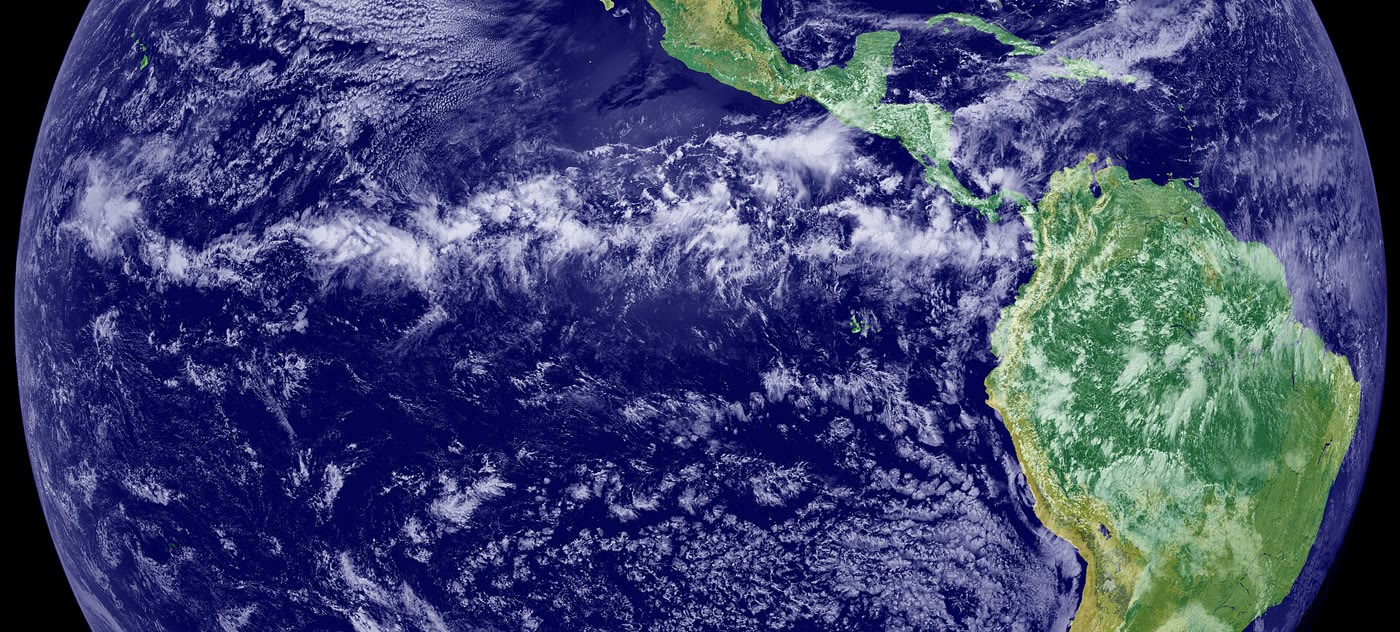
\includegraphics[width=0.8\linewidth]{images/book3/b1-itcz-goes.jpg}

{\small De \omterm{def:b1:atmospheric-circulation:itcz}{intertropische convergentiezone} boven de oostelijke Stille Oceaan: een lijn van heldere wolken die de oceaan ten noorden van de evenaar doorkruist, met Midden- en Zuid-Amerika rechts. Het beeld combineert wolkendata van de geostationaire satelliet GOES-11 met kleuren van de landbedekking. (NASA Earth Observatory, publiek domein, via Wikimedia Commons.)}
\label{fig:b1:atmospheric-circulation:itcz-photo}
\end{omfigure}
% ledger: commons:itcz-goes

Convergerende lucht moet stijgen, en opstijgende vochtige lucht bouwt wolken op: de ITCZ is de regenrijkste gordel van de planeet, en haar positie wordt gemeten als de \omterm{def:b1:spherical-astronomy:geographic}{breedtegraad} waar de zonaal gemiddelde neerslag haar maximum bereikt. De ITCZ volgt de zon, met vertraging. In de reanalyse verschuift het maximum van \ang{12.8} Z in februari naar \ang{10.9} N in september; over de twaalf maanden gemiddeld ligt het op \ang{2.6} N. Het zonaal gemiddelde verbergt grote verschillen tussen de lengtegraden: boven de oostelijke Stille Oceaan op de foto ligt de band ten noorden van de evenaar, en een zonaal gemiddelde middelt zulke banden met andere die met de seizoenen verder zwaaien.
% ledger: data:b3-ncep (computed in figdata/bachelor-1/general_circulation.py)

\begin{omfigure}
\begin{tikzpicture}
\begin{axis}[omrecord, width=0.7\linewidth, height=5.2cm, xmin=0.5, xmax=12.5, ymin=-16, ymax=16,
  xlabel={maand}, ylabel={breedtegraad (\unit{\degree})}, xtick={1,...,12},
  xticklabels={J,F,M,A,M,J,J,A,S,O,N,D}, ytick={-15,-10,...,15}]
% figdata/bachelor-1/general_circulation.py; ledger: data:b3-ncep
\addplot[black!40, domain=0.5:12.5] {0};
\addplot[omThm, line width=1.1pt, mark=*, mark size=1.6pt] table[x=month, y=lat] {figdata/out/bachelor-1-general_circulation-itcz.dat};
\end{axis}
\end{tikzpicture}

{\small De \omterm{def:b1:spherical-astronomy:geographic}{breedtegraad} van het maximum van de zonaal gemiddelde neerslag, maand voor maand, tussen \ang{20} Z en \ang{20} N: de \omterm{def:b1:atmospheric-circulation:itcz}{intertropische convergentiezone} trekt in de noordelijke zomer naar het noorden en in de zuidelijke zomer naar het zuiden, twee of drie maanden achter de zon.
NCEP-NCAR Reanalysis~1, gemiddelden 1991--2020, gegevens verstrekt door de NOAA PSL.}
\label{fig:b1:atmospheric-circulation:itcz}
\end{omfigure}
% ledger: data:b3-ncep

Langs de evenaar zelf, waar $f = 0$, beweegt de lucht recht in de richting van de lagere druk, en verschijnt boven de Stille Oceaan een oost-westcirculatie.

\begin{definition}[Walkercirculatie]\label{def:b1:atmospheric-circulation:walker}
De \emph{Walkercirculatie}\index{Walkercirculatie} is de oost-westelijke overturningscel van de atmosfeer langs de equatoriale Stille Oceaan: lucht stijgt boven de warme wateren van het westen, rond het Maritiem Continent,
stroomt hoog naar het oosten, daalt boven de oostelijke Stille Oceaan en keert aan het oppervlak naar het westen terug met de \omterm{def:b1:atmospheric-circulation:winds}{passaten}.
\end{definition}
% ledger: climategov:walker

\begin{omfigure}
\begin{tikzpicture}[>={Stealth[length=2mm]}, font=\scriptsize]
  \fill[blue!12] (0,0) rectangle (11,0.45);
  \shade[left color=orange!45, right color=blue!12] (0,0) rectangle (6,0.45);
  \fill[brown!45] (-0.9,0) rectangle (0,0.6);
  \fill[brown!45] (11,0) rectangle (11.9,0.6);
  \node[anchor=north] at (-0.45,-0.05) {Maritiem};
  \node[anchor=north] at (-0.45,-0.35) {Continent};
  \node[anchor=north] at (11.45,-0.05) {Zuid-};
  \node[anchor=north] at (11.45,-0.35) {Amerika};
  \node[anchor=north] at (5.5,-0.05) {equatoriale Stille Oceaan};
  \node at (1.6,0.22) {warm water};
  \foreach \x in {0.6,1.2,1.8} \fill[black!20] (\x,2.6) circle (0.45);
  \foreach \x in {0.9,1.5} \fill[black!25] (\x,3.0) circle (0.4);
  \draw[line width=1.2pt, omThm, ->] (9.5,0.8) -- (2.0,0.8);
  \draw[line width=1.2pt, omThm, ->] (1.2,1.0) -- (1.2,3.0);
  \draw[line width=1.2pt, omThm, ->] (2.0,3.3) -- (9.5,3.3);
  \draw[line width=1.2pt, omThm, ->] (10.3,3.0) -- (10.3,1.0);
  \node[anchor=south] at (5.75,0.85) {passaten, van oost naar west};
  \node[anchor=south] at (5.75,3.35) {terugstroom hoog, van west naar oost};
  \node[anchor=west, align=left] at (1.6,1.8) {stijgende lucht,\\zware regen};
  \node[anchor=east, align=right] at (10.0,1.8) {dalende lucht,\\droog};
\end{tikzpicture}

{\small De \omterm{def:b1:atmospheric-circulation:walker}{Walkercirculatie} langs de equatoriale Stille Oceaan (schematisch; hoogte niet op schaal): stijgend boven het warme westen, hoog naar het oosten, dalend in het oosten en aan het oppervlak weer naar het westen met de \omterm{def:b1:atmospheric-circulation:winds}{passaten}.}
\label{fig:b1:atmospheric-circulation:walker}
\end{omfigure}
% ledger: climategov:walker

De \omterm{def:b1:atmospheric-circulation:walker}{Walkercirculatie} is niet stabiel. Wanneer zij verzwakt, neemt de opstijging boven het Maritiem Continent af en kan de lucht daar zelfs dalen; wanneer zij versterkt, nemen de opstijging en de regen boven het westen toe. Deze schommelingen, El~Niño en La~Niña, en de seizoensomkeringen van de moessons zijn het onderwerp van Boek~4.
Over de decennia sinds 1980 vindt het IPCC-rapport uit 2021 een \emph{zeer waarschijnlijke} versterking van de \omterm{def:b1:atmospheric-circulation:walker}{Walkercirculatie}, die lijkt op de La~Niña-toestand, en een verschuiving naar het westen, met \emph{gemiddeld vertrouwen} in de omvang van de veranderingen.
% ledger: climategov:walker, ipcc:hadley-widening

\section{Straalstromen}\label{sec:b1:atmospheric-circulation:jets}

\begin{definition}[Straalstroom; subtropische en poolfront-straalstromen]\label{def:b1:atmospheric-circulation:jet}
Een \emph{straalstroom}\index{straalstroom} is een smalle band van sterke wind, meestal een horizontale wind hoog in de troposfeer, waarvan de positie van dag tot dag verandert. De \emph{subtropische straalstroom}\index{subtropische straalstroom} waait uit het westen nabij de poolwaartse rand van de \omterm{def:b1:atmospheric-circulation:cells}{Hadley-cel}, meestal tussen \ang{20} en \ang{30} \omterm{def:b1:spherical-astronomy:geographic}{breedtegraad} op hoogten van \qtyrange{12}{14}{km}. De \emph{poolfront-straalstroom}\index{poolfront-straalstroom} waait uit het westen boven de grens tussen poolse en subtropische lucht, tussen ongeveer \ang{50} en \ang{60}; zij is de snelle kern van de \omterm{def:b1:atmospheric-circulation:winds}{westenwinden}, gestuurd door en sturend voor de depressies en anticyclonen van de middelbreedten.
\end{definition}
% ledger: nws:jets, noaajs:jet

Straalstromen worden doorgaans rond \qty{9}{km} gevonden, kunnen meer dan \qty{440}{km/h} bereiken en zijn het sterkst in de winter van elk halfrond, wanneer het temperatuurcontrast tussen de tropen en de pool het grootst is. De \omterm{def:b1:atmospheric-circulation:jet}{subtropische straalstroom} is de impulsmomentwind van
\cref{prop:b1:atmospheric-circulation:angular-momentum}, getemd door de wervels; zij ligt aan de rand van de \omterm{def:b1:atmospheric-circulation:cells}{Hadley-cel}, nabij \ang{30} in het winterse gemiddelde. De \omterm{def:b1:atmospheric-circulation:jet}{poolfront-straalstroom} zwerft noord en zuid met de voorbijtrekkende depressies, en het middelen over de hele aarde vervaagt haar: in het zonaal gemiddelde van de noordelijke zomer blijft slechts een zwak maximum van \qty{21.6}{m/s} over nabij \ang{42.5} N, en in de zuidelijke zomer \qty{29.9}{m/s} nabij \ang{47.5} Z. Waarom de wind toeneemt met de hoogte waar de temperatuur naar de pool daalt, de thermische wind, wordt behandeld in Boek~5.
% ledger: noaajs:jet, nws:jets, data:b3-ncep-circ (computed in figdata/bachelor-1/general_circulation.py)

\section{Oefeningen}

\begin{exercise}[$\star$]\label{exo:b1:atmospheric-circulation:1}
Neem $\Omega = \qty{7.292e-5}{rad.s^{-1}}$. (a)~Bereken de \omterm{def:b1:atmospheric-circulation:coriolis-parameter}{Coriolisparameter} op
\ang{0}, \ang{30}, \ang{45} en \ang{90} N. (b)~Bereken de horizontale Coriolisversnelling
van een wind van \qty{10}{m/s} op \ang{45} N en vergelijk haar met $g =
\qty{9.81}{m.s^{-2}}$. (c)~In welke richting wijst zij als de wind naar het noorden waait?
% ledger: earth:Trot
\end{exercise}

\begin{exercise}[$\star$]\label{exo:b1:atmospheric-circulation:2}
Twee isobaren die \qty{4}{hPa} van elkaar liggen, staan op zeeniveau \qty{400}{km} uit elkaar, waar $\rho =
\qty{1.225}{kg.m^{-3}}$. (a)~Bereken de versnelling door de \omterm{def:b1:atmospheric-circulation:pgf}{drukgradiëntkracht}. (b)~Als er niets anders werkte, hoe lang zou het duren om stille lucht op
\qty{10}{m/s} te versnellen? (c)~Vergelijk deze versnelling met de Coriolisversnelling van een wind van
\qty{10}{m/s} op \ang{45} N, en zeg wat dit suggereert.
% ledger: ussa76:sea-level, earth:Trot
\end{exercise}

\begin{exercise}[$\star$]\label{exo:b1:atmospheric-circulation:3}
Op \ang{40} N staan isobaren die \qty{4}{hPa} uit elkaar liggen \qty{250}{km} van elkaar; neem $\rho =
\qty{1.225}{kg.m^{-3}}$. (a)~Bereken de \omterm{def:b1:atmospheric-circulation:geostrophic}{geostrofische wind} in \unit{m/s} en in knopen
(\qty{1}{kn} = \qty{0.5144}{m/s}). (b)~De lage druk ligt in het zuiden. Uit welke
richting waait de wind? (c)~Beschrijf de windpen (staf en veren) die een weerkundige zou tekenen.
% ledger: ussa76:sea-level, earth:Trot
\end{exercise}

\begin{exercise}[$\star$]\label{exo:b1:atmospheric-circulation:4}
De jaargemiddelden van de reanalyse geven, nabij de grond, de oostelijke wind
\qty{-3.5}{m/s} op \ang{15} N, \qty{-4.4}{m/s} op \ang{15} Z, \qty{+1.9}{m/s} op
\ang{45} N en \qty{+6.5}{m/s} op \ang{45} Z, en de zeeniveaudruk
\qty{1011.8}{hPa} op \ang{15} N, \qty{1016.8}{hPa} op \ang{30} N en
\qty{1015.8}{hPa} op \ang{45} N. (a)~Benoem de windgordel op elk van de vier breedtegraden.
(b)~Verklaar het teken van elke wind met de oppervlaktetak van een cel. (c)~Waar ligt volgens deze drukken de subtropische hogedrukgordel van het noordelijk halfrond?
% ledger: data:b3-ncep-circ
\end{exercise}

\begin{exercise}[$\star\star$]\label{exo:b1:atmospheric-circulation:5}
Een drukgradiënt van \qty{2}{hPa} per \qty{500}{km}, met $\rho =
\qty{1.225}{kg.m^{-3}}$, wordt aangetroffen op \ang{60}, \ang{50}, \ang{30}, \ang{20},
\ang{10} en \ang{5} N. (a)~Bereken de \omterm{def:b1:atmospheric-circulation:geostrophic}{geostrofische wind} op elke \omterm{def:b1:spherical-astronomy:geographic}{breedtegraad}.
(b)~Echte winden in de diepe tropen overschrijden boven zulke gradiënten zelden enkele meters per seconde. Verklaar waarom de geostrofische balans nabij de evenaar faalt, met de tijd $1/f$ die de Coriolis-kracht nodig heeft om de wind te draaien.
% ledger: ussa76:sea-level, earth:Trot
\end{exercise}

\begin{exercise}[$\star\star$]\label{exo:b1:atmospheric-circulation:6}
(a)~Bereken met \cref{prop:b1:atmospheric-circulation:angular-momentum} de wind
van een ring lucht die de evenaar in rust verlaat, op \ang{10}, \ang{15}, \ang{20} en
\ang{30}; neem $\Omega a_\oplus = \qty{464.6}{m/s}$. (b)~Hetzelfde voor een ring die
in rust begint op \ang{10}, \ang{15}, \ang{20} en \ang{30}. (c)~De opstijgende tak
van de \omterm{def:b1:atmospheric-circulation:cells}{Hadley-cel} is over breedtegraden verspreid in plaats van precies op de evenaar gelegen.
Hoe verandert dit de voorspelde \omterm{def:b1:atmospheric-circulation:jet}{straalstroom}?
% ledger: earth:Trot, earth:Rmean
\end{exercise}

\begin{exercise}[$\star\star$]\label{exo:b1:atmospheric-circulation:7}
(a)~Een schip op het noordelijk halfrond heeft de wind uit het zuidwesten. Waar ligt volgens de wet van Buys Ballot het centrum van de lage druk? (b)~Een schip op het zuidelijk halfrond heeft de wind uit het noordwesten. Waar ligt de lage druk? (c)~Nabij de grond snijdt de wind de isobaren naar lage druk. Verandert dit het antwoord op (a), en zo ja, draait de richting van de lage druk dan rechtsom of linksom?
% ledger: skybrary:buys-ballot
\end{exercise}

\begin{exercise}[$\star\star$]\label{exo:b1:atmospheric-circulation:8}
(a)~Bereken de massa lucht tussen de evenaar en \ang{30} N en tussen de drukniveaus
\qty{1000}{hPa} en \qty{100}{hPa}, met $a_\oplus = \qty{6371}{km}$
en $g = \qty{9.81}{m.s^{-2}}$. (b)~In het jaargemiddelde draagt de noordelijke
\omterm{def:b1:atmospheric-circulation:cells}{Hadley-cel} van de reanalyse \qty{8.7e10}{kg/s}. Hoe lang duurt het om die massa eenmaal door de cel te laten gaan? (c)~Dezelfde vraag voor de cel van de noordelijke winter, \qty{21.4e10}{kg/s}.
% ledger: earth:Rmean, data:b3-ncep-circ
\end{exercise}

\begin{exercise}[$\star\star$]\label{exo:b1:atmospheric-circulation:9}
Veronderstel dat onder een subtropische hogedrukgordel de lucht daalt met \qty{1}{cm/s}, en dat zij onverzadigd is. (a)~Hoe ver daalt zij in een dag? (b)~Hoeveel warmt zij in een dag op, als er verder niets werkt, met de \omterm{def:b1:fluid-envelopes-structure:lapse-rate}{droogadiabatische gradiënt} van \qty{9.8}{K/km}? (c)~De lucht warmt niet dag na dag zoveel op. Welk proces van \cref{ch:b1:radiation-heat-transport} houdt de opwarming in evenwicht? (d)~Waarom liggen veel van de grote hete woestijnen onder deze hogedrukgebieden?
% ledger: nws:dalr
\end{exercise}

\begin{exercise}[$\star\star\star$]\label{exo:b1:atmospheric-circulation:10}
Neem op \ang{50} N $f = \qty{1.117e-4}{s^{-1}}$ en cirkelvormige isobaren met straal
$r = \qty{500}{km}$ (\cref{rem:b1:atmospheric-circulation:gradient}). (a)~Rond
een lage druk waar de \omterm{def:b1:atmospheric-circulation:geostrophic}{geostrofische wind} \qty{15}{m/s} zou zijn, los $V^2/r + fV =
f|\vec v_g|$ op voor de gradiëntwind $V$. (b)~Rond een hoge druk toon aan dat $V^2/r - fV + f
|\vec v_g| = 0$ slechts een oplossing heeft als $|\vec v_g| \leq fr/4$, en bereken die grens.
(c)~Wat impliceert (b) voor de afstand tussen de isobaren nabij het centrum van een
\omterm{def:b1:atmospheric-circulation:cyclone}{anticycloon}, vergeleken met een depressie?
\end{exercise}

\begin{exercise}[$\star\star\star$]\label{exo:b1:atmospheric-circulation:11}
(a)~Toon aan dat voor kleine $\varphi$ (in radialen) de wind van een ring die de evenaar in rust verlaat
gelijk is aan $u \approx \Omega a_\oplus\varphi^2$. (b)~Vergelijk de benadering met
de exacte formule op \ang{10}, met $\Omega a_\oplus = \qty{464.6}{m/s}$. (c)~De
jaargemiddelde wind van de reanalyse op \qty{200}{hPa} piekt op \qty{27.0}{m/s} nabij
\ang{35} N. Op welke \omterm{def:b1:spherical-astronomy:geographic}{breedtegraad} zou de ring deze snelheid bereiken? (d)~Wat zegt het antwoord over hoe ver het impulsmomentargument te vertrouwen is?
% ledger: earth:Trot, earth:Rmean, data:b3-ncep-circ
\end{exercise}

\begin{exercise}[$\star\star\star$]\label{exo:b1:atmospheric-circulation:12}
De zonaal gemiddelde neerslagmaxima van de reanalyse liggen op de volgende
breedtegraden, van januari tot december: \ang{-10.5}, \ang{-12.8}, \ang{-5.8}, \ang{-4.6}, \ang{5.5},
\ang{7.3}, \ang{8.6}, \ang{10.4}, \ang{10.9}, \ang{9.1}, \ang{7.4}, \ang{6.2}
(negatief: zuid). (a)~Bereken het jaargemiddelde en de spreiding. (b)~De subsolaire \omterm{def:b1:spherical-astronomy:geographic}{breedtegraad} bereikt haar uiterste waarden in juni en december. Met hoeveel maanden loopt de ITCZ erachter aan, en wat in het klimaatsysteem kan warmte opslaan om zo'n vertraging te veroorzaken? (c)~Veronderstel dat boven één oceaan de ITCZ het hele jaar ten noorden van de evenaar blijft. Leg uit hoe het zonaal gemiddelde de evenaar toch kan kruisen.
% ledger: data:b3-ncep
\end{exercise}

\section{Probleem: een weerkaart van de middelbreedten lezen}

\begin{problem}[{Weekendprobleem --- de wind op een station nabij \ang{50} N}]
\label{pb:b1:atmospheric-circulation:1}
% values: calc/ch28.py (invented map; jet from data:b3-ncep-circ)
Een weerkaart van de Noord-Atlantische Oceaan toont, nabij een station P op \ang{50} N, rechte isobaren die van west naar oost lopen, elke \qty{4}{hPa}, met de lagere drukken naar het noorden. P ligt tussen de isobaren van \qty{1004}{hPa} en \qty{1008}{hPa}, die daar \qty{250}{km} uit elkaar liggen; de zeeniveaudruk is er \qty{1006}{hPa} en de luchttemperatuur \qty{10}{\degreeCelsius}. De kaart is verzonnen, maar haar getallen zijn gebruikelijk.
Gebruik $\Omega = 2\pi/(\qty{23.9345}{h})$, $a_\oplus = \qty{6371}{km}$, $R_d =
\qty{287.05}{J.kg^{-1}.K^{-1}}$ voor droge lucht, \qty{1}{kn} = \qty{0.514444}{m/s}.

\medskip
\noindent\textbf{Deel I --- De drukgradiënt en de geostrofische wind.}
\begin{enumerate}
  \item Bereken de dichtheid van de lucht op P met de wet van de ideale gassen.
  \item Bereken de horizontale drukgradiënt op P, in \unit{Pa.m^{-1}}.
  \item Bereken de versnelling door de \omterm{def:b1:atmospheric-circulation:pgf}{drukgradiëntkracht}.
  \item Bereken $\Omega$ en de \omterm{def:b1:atmospheric-circulation:coriolis-parameter}{Coriolisparameter} op \ang{50} N.
  \item Bereken de snelheid van de \omterm{def:b1:atmospheric-circulation:geostrophic}{geostrofische wind} op P.
  \item Druk die uit in knopen en in \unit{km/h}.
  \item Toon aan dat de tijd die de \omterm{def:b1:atmospheric-circulation:pgf}{drukgradiëntkracht} alleen nodig heeft om stille lucht op de geostrofische snelheid te brengen $1/f$ is, en bereken die, samen met
        de tijd $2\pi/f$ die de Coriolis-kracht nodig heeft om een wind een volle cirkel te laten draaien.
\end{enumerate}

\medskip
\noindent\textbf{Deel II --- Richting en halfrond.}
\begin{enumerate}[resume]
  \item In welke richting wijst de \omterm{def:b1:atmospheric-circulation:pgf}{drukgradiëntkracht} op P? In welke
        richting waait de \omterm{def:b1:atmospheric-circulation:geostrophic}{geostrofische wind}, en vanaf welke \omterm{def:b1:spherical-astronomy:horizontal}{azimut} komt zij?
  \item Controleer het antwoord met de wet van Buys Ballot.
  \item Beschrijf de windpen die op P is getekend: de richting van de staf, het aantal veren en de zijde waaraan zij staan.
  \item Veronderstel dat dezelfde isobaren, met de lage druk ten noorden, op \ang{50} Z zouden worden aangetroffen. Uit welke richting zou de wind waaien?
  \item Bereken met dezelfde dichtheid en drukgradiënt de \omterm{def:b1:atmospheric-circulation:geostrophic}{geostrofische wind} op \ang{30} N en \ang{60} N.
  \item Bereken hem op \ang{5} N. Is het resultaat geloofwaardig? Leg uit.
\end{enumerate}

\medskip
\noindent\textbf{Deel III --- De wind aan de grond.} Een windmeter op P meet een
wind van \qty{9.0}{m/s} die de isobaren snijdt onder \ang{25} naar lage druk toe.
\begin{enumerate}[resume]
  \item Bereken de verhouding van de waargenomen wind tot de \omterm{def:b1:atmospheric-circulation:geostrophic}{geostrofische wind}, en de
        componenten van de waargenomen wind langs en dwars op de isobaren.
  \item Uit welke \omterm{def:b1:spherical-astronomy:horizontal}{azimut} waait de waargenomen wind?
  \item In het lineaire wrijvingsmodel van \cref{prop:b1:atmospheric-circulation:friction},
        welke tijdconstante $\tau$ geeft de waargenomen hoek, en welke snelheid voorspelt het
        model dan? Vergelijk met de waarneming.
  \item Veronderstel rond een depressie met straal \qty{500}{km} dat de lucht van de
        laagste kilometer overal naar binnen stroomt met de component dwars op de isobaren uit
        vraag~14 en de dichtheid uit vraag~1. Bereken de massa lucht die per seconde
        de depressie binnenstroomt.
  \item Deze lucht moet door de bovenkant van de laag weg. Bereken de gemiddelde opwaartse
        snelheid daar, in \unit{m/s} en in meter per dag.
  \item Hoeveel koelt de opstijgende lucht in een dag af bij de \omterm{def:b1:fluid-envelopes-structure:lapse-rate}{droogadiabatische gradiënt} van \qty{9.8}{K/km}? Welk weer volgt, en wat zou er
        onder een \omterm{def:b1:atmospheric-circulation:cyclone}{anticycloon} in plaats daarvan gebeuren?
\end{enumerate}

\medskip
\noindent\textbf{Deel IV --- De straalstroom erboven.} De zonaal gemiddelde wind op \qty{200}{hPa} in
de noordelijke winter piekt op \qty{42.3}{m/s} nabij \ang{30} N (gemiddelden van de reanalyse
1991--2020).
\begin{enumerate}[resume]
  \item Bereken de oostelijke snelheid van de grond op de evenaar en op \ang{30} N.
  \item Een ring lucht verlaat de evenaar in rust hoog in de atmosfeer en behoudt haar impulsmoment. Bereken haar wind op \ang{20} N en \ang{30} N.
  \item Zelfde vraag op \ang{30} N voor een ring die in rust begint op \ang{10} N.
  \item Met welke factor loopt de ring uit vraag~21 de waargenomen \omterm{def:b1:atmospheric-circulation:jet}{straalstroom} op \ang{30} N voor? Geef twee redenen waarom de werkelijke \omterm{def:b1:atmospheric-circulation:jet}{straalstroom} trager is.
  \item Bereken de verhouding van het absolute impulsmoment per massa-eenheid van de waargenomen \omterm{def:b1:atmospheric-circulation:jet}{straalstroom} op \ang{30} N tot dat van lucht in rust op de evenaar. Welk deel is onderweg verloren gegaan?
  \item Hoe groot is de geostrofische windsnelheid op P, in meter per seconde, en hoe verhoudt de aan de grond gemeten wind zich daarmee?
\end{enumerate}
\end{problem}
